% Options for packages loaded elsewhere
\PassOptionsToPackage{unicode}{hyperref}
\PassOptionsToPackage{hyphens}{url}
%
\documentclass[
]{article}
\usepackage{amsmath,amssymb}
\usepackage{iftex}
\ifPDFTeX
  \usepackage[T1]{fontenc}
  \usepackage[utf8]{inputenc}
  \usepackage{textcomp} % provide euro and other symbols
\else % if luatex or xetex
  \usepackage{unicode-math} % this also loads fontspec
  \defaultfontfeatures{Scale=MatchLowercase}
  \defaultfontfeatures[\rmfamily]{Ligatures=TeX,Scale=1}
\fi
\usepackage{lmodern}
\ifPDFTeX\else
  % xetex/luatex font selection
\fi
% Use upquote if available, for straight quotes in verbatim environments
\IfFileExists{upquote.sty}{\usepackage{upquote}}{}
\IfFileExists{microtype.sty}{% use microtype if available
  \usepackage[]{microtype}
  \UseMicrotypeSet[protrusion]{basicmath} % disable protrusion for tt fonts
}{}
\makeatletter
\@ifundefined{KOMAClassName}{% if non-KOMA class
  \IfFileExists{parskip.sty}{%
    \usepackage{parskip}
  }{% else
    \setlength{\parindent}{0pt}
    \setlength{\parskip}{6pt plus 2pt minus 1pt}}
}{% if KOMA class
  \KOMAoptions{parskip=half}}
\makeatother
\usepackage{xcolor}
\usepackage[margin=1in]{geometry}
\usepackage{longtable,booktabs,array}
\usepackage{calc} % for calculating minipage widths
% Correct order of tables after \paragraph or \subparagraph
\usepackage{etoolbox}
\makeatletter
\patchcmd\longtable{\par}{\if@noskipsec\mbox{}\fi\par}{}{}
\makeatother
% Allow footnotes in longtable head/foot
\IfFileExists{footnotehyper.sty}{\usepackage{footnotehyper}}{\usepackage{footnote}}
\makesavenoteenv{longtable}
\usepackage{graphicx}
\makeatletter
\def\maxwidth{\ifdim\Gin@nat@width>\linewidth\linewidth\else\Gin@nat@width\fi}
\def\maxheight{\ifdim\Gin@nat@height>\textheight\textheight\else\Gin@nat@height\fi}
\makeatother
% Scale images if necessary, so that they will not overflow the page
% margins by default, and it is still possible to overwrite the defaults
% using explicit options in \includegraphics[width, height, ...]{}
\setkeys{Gin}{width=\maxwidth,height=\maxheight,keepaspectratio}
% Set default figure placement to htbp
\makeatletter
\def\fps@figure{htbp}
\makeatother
\usepackage{soul}
\setlength{\emergencystretch}{3em} % prevent overfull lines
\providecommand{\tightlist}{%
  \setlength{\itemsep}{0pt}\setlength{\parskip}{0pt}}
\setcounter{secnumdepth}{-\maxdimen} % remove section numbering
\ifLuaTeX
  \usepackage{selnolig}  % disable illegal ligatures
\fi
\IfFileExists{bookmark.sty}{\usepackage{bookmark}}{\usepackage{hyperref}}
\IfFileExists{xurl.sty}{\usepackage{xurl}}{} % add URL line breaks if available
\urlstyle{same}
\hypersetup{
  pdftitle={SOBRE LOS PRINCIPIOS TRIBUTARIOS},
  pdfauthor={Tomàs Ferrandis Moscardó},
  hidelinks,
  pdfcreator={LaTeX via pandoc}}

\title{SOBRE LOS PRINCIPIOS TRIBUTARIOS}
\author{Tomàs Ferrandis Moscardó}
\date{2022-12-16}

\begin{document}
\maketitle

{
\setcounter{tocdepth}{2}
\tableofcontents
}
\hypertarget{introducciuxf3n}{%
\section*{1 INTRODUCCIÓN}\label{introducciuxf3n}}
\addcontentsline{toc}{section}{1 INTRODUCCIÓN}

El objetivo de este trabajo es mostrar la importancia de los principios
tributarios estudiados en la asignatura Economía Pública (Tema 8.
Epígrafe 8.5. Los principios tributarios) tanto en el sistema impositiva
actual y su debate.

En un primer punto expondremos la visión crítica sobre nuestro sistema
impositivo compartida por catedráticos de Derecho Financiero y
Tributario españoles. También veremos una crítica basada en los
principios que debe seguir un tributario para ser óptimo según el premio
Nobel Mirrlees. Ambas visiones, distintas en muchos aspectos, y por ello
escogidas, coincidirán en demandar una mayor atención a algunos
principios. Verbigracia, la demanda de una mayor simplicidad y un cambio
en el trato dado son una constante en todas opiniones consultadas sobre
nuestro sistema impositivo.

En un segundo apartado abordaremos la importancia o el sentido de los
principios presupuestarios cuando nos planteamos los impuestos como
instrumentos para cambiar, desde hábitos de consumo a modelos de
producción. Hablaremos de los recientes impuestos verdes establecidos,
no para recaudar, sino para afrontar los retos ineludibles sobre el
medioambiente. ¿Se puede cambiar el modelo de economía lineal y energía
contaminante sin abandonar la idea liberal ser ``neutral'' ?, ¿qué
sentido tiene la eficiencia o suficiencia?

La tercera parte hará referencia a otro principio fundamental, el de la
equidad, aunque relacionado con el resto de principios, fundamentalmente
el de suficiencia y el de neutralidad. Analizaremos la visión
socialdemócrata y la liberal. Para entender el razonamiento de cada
planteamiento expondremos el caso real de Irlanda y la propuesta de
nuevo impuesto del economista Thomas Piketty. ¿ Eficiencia derivada de
la neutralidad y transferencias, o justicia basada en la progresividad e
impuestos directos sobre el capital ?

En un último apartado, atenderemos a la reciente aprobación de impuestos
excepcionales en Esapña. El debate que se ha cernido sobre cada uno de
ellos pivotaba, también, sobre los principios del sistema tributarios
objeto de estudio.

Así pues, en este trabajo se ha pretendido poner el foco en el
cuestionamiento y la defensa de los principios tributarios en nuestro
contexto más actual.

\hypertarget{ciudadanos-o-suxfabditos}{%
\section*{2 ¿CIUDADANOS O SÚBDITOS?}\label{ciudadanos-o-suxfabditos}}
\addcontentsline{toc}{section}{2 ¿CIUDADANOS O SÚBDITOS?}

En este tema hemos visto los principios que pueden regir, o no, en un
determinado sistema impositivo en general. En el presente apartado vamos
a contextualizar y exponer dos visiones críticas con nuestro actual
sistema tributario donde se compartirán gran parte de dichos principios.
Por una parte, la conocida como Declaración de Granada y, en segundo
lugar, reflexiones de la economista Anna Rossell basadas en las
conclusiones del informe Mirrlees (Rossell, 2020).

\hypertarget{la-declaraciuxf3n-de-granada}{%
\subsection*{2.1 LA DECLARACIÓN DE
GRANADA}\label{la-declaraciuxf3n-de-granada}}
\addcontentsline{toc}{subsection}{2.1 LA DECLARACIÓN DE GRANADA}

En 2018, treinta y cinco catedráticos españoles de Derecho Financiero y
Tributario firmaron un manifiesto demoledor contra el sistema tributario
español ( Rodríguez, 2018). La conocida como Declaración de Granada
arranca con una defensa del papel de los tributos y una advertencia
sobre el peligro del fraude tributario. Así pues, denuncian las reglas
del juego que facilitan a las grandes compañías, sobre todo las que
prestan servicios on-line, esquivar los impuestos ``forzando sus reglas
de aplicación espacial'', así como aquellas que les permiten concertar
con la Administración determinados regímenes fiscales favorables.

Al margen de todo, según los catedráticos, este hecho no puede ocultar
ni excusar el exceso de afán recaudatorio que llega a dejar de lado los
derechos y garantías (incluso constitucionales) de los ciudadanos.

De forma sumaria exponemos sus principales argumentos de los firmantes.

\textbf{Quiebra del principio de legalidad y abuso de poder}

Manifiestan su rechazo al desplazamiento del poder legislativo por parte
del poder ejecutivo mediante el abuso de la figura del Decreto-Ley. Esta
una perversión del Estado de Derecho no se produce solo en el ámbito
tributario. Desgraciadamente es una práctica cada día más extendida:
legislar a golpe de ``urgente necesidad'' en todos los ámbitos.

Otra crítica afecta al abandono de la interpretación de la norma por
parte del Tribunal Constitucional, sobre todo, al asumir la
``jurisprudencia'' como fuente de derecho por haber asumido sin crítica
la función normativa del Tribunal de Justicia de la Unión Europea.

Además, lamentan la actitud del legislador que olvida la necesidad de
hacerse entender en sus textos, cambia las normas cuando las sentencias
judiciales no son de su agrado y, lo que es más grave, en los
procedimientos que establece siempre parte de la presunción de
culpabilidad del ciudadano en vez de la presunción de inocencia.

\textbf{Quiebra del principio de igualdad}

La igualdad no solo afecta de forma horizontal entre los ciudadanos
obligándonos a todos a contribuir, sino también en un sentido vertical
estableciendo una exigencia de acuerdo a la capacidad de cada miembro de
la comunidad. Contrariamente se ha llegado a concebir la responsabilidad
tributaria como algo ajeno a la obligación del sujeto pasivo que puede
extenderse a otra persona, física o jurídica. La finalidad de recaudar
de manera práctica y rápida lo justifica ya todo. Aparece la figura del
``deudor solidario'' que, pese a no tener vinculación con el hecho
imponible, acaba pagando.

La perversión del principio de colaboración del contribuyente también la
ven como ejemplo de esta quiebra de principios. Se practica la
liquidación de oficio y no se asiste al contribuyente en nada más que en
el procedimiento sancionador. Además se le fuerza a declarar en su
contra vulnerando un derecho constitucional. Todo ello, al margen de que
haya un procedimiento penal paralelo.

\textbf{La quiebra del sentido de seguridad jurídica}

Este problema lo hemos tratado en el tema, al tratar el principio de
simplicidad que no se cumple ni para la misma administración tributaria.
En el mimo sentido, los firmantes de la Declaración denuncian que en
cada autonomía se siguen unos criterios distintos atendiendo a sus
necesidades, lo que significa, según ellos, una quiebra del principio de
igualdad. Reclaman la solidaridad que exige la Constitución basada en
una coordinación de las Haciendas autonómicas con la Hacienda estatal.

\textbf{Quiebra del principio de justicia financiera}

En el ámbito de los ingresos, la deuda pública debería ser un ingreso
excepcional. Por el contrario, se ha convertido en un ingreso ordinario,
trasladándose sobre generaciones futuras el coste de financiar servicios
actuales.

En el ámbito de los gastos, los firmantes, además de alertar sobre la
falta de control jurídico en el gasto público, atacan el mercadeo que se
produce, según ellos, en sede parlamentaria para conseguir los votos
necesarios para la aprobación del Presupuesto General del Estado.
Critican el abuso del poder ejecutivo, no solo a través de los
Decretos-leyes, sino también en el veto a propuestas que impliquen un
aumento de gastos o disminución de ingresos.

La conclusión de los catedráticos es que la Hacienda Pública se ha
convertido en un agente dedicado, y motivado, exclusivamente por y para
la recaudación, quebrantando el principio de legalidad, apartándose de
la función de la Ley y de las Cortes Generales, lo que, en un Estado de
Derecho, supone una erosión de la seguridad jurídica.

\hypertarget{un-buen-sistema-impositivo}{%
\subsection*{2.2 UN BUEN SISTEMA
IMPOSITIVO}\label{un-buen-sistema-impositivo}}
\addcontentsline{toc}{subsection}{2.2 UN BUEN SISTEMA IMPOSITIVO}

Ante la pregunta de cuál es el nivel de ingresos necesario en un Estado
de bienestar nos asalta otra: ¿cuál es la forma más eficiente de poder
recaudar estos ingresos? Evidentemente que la respuesta a la primera
pregunta es algo que depende de la capacidad de nuestro país, pero en el
caso de la segunda, entramos en el terreno del debate sobre los
principios presupuestarios.

Para aclarar esta cuestión la economista Anna Rossell recurren al
Informe de Mirrlees y defienden cinco principios como ejes de un sistema
fiscal óptimo (Rossell, 2020). Estos principios serían:

\begin{itemize}
\item
  Eficiencia
\item
  Minimización de costes
\item
  Simplicidad y transparencia
\item
  Progresividad
\item
  Imparcialidad
\end{itemize}

\textbf{Eficiencia}

Se entiende ésta como una consecuencia de la ya estudiada en la
asignatura ``neutralidad de los tributos''.

Los datos aportados por la profesora Rossell se basan en simulaciones
(Boscá, Doménech y Ferri, 2017) según los cuales el aumento de un punto
porcentual sobre el PIB del IVA haría caer el PIB 0,75 puntos, en
cambio, el aumento del IRPF en la misma proporción deprimiría el PIB en
0,84 puntos; el aumento en las cotizaciones a la Seguridad Social
supondría una caída de 1 punto y el aumento en la tributación sobre el
capital haría disminuir el PIB en 1,22 puntos.

La conclusión de estos estudios es que un sistema basado en impuestos
directos sobre consumo es más neutral que el basado en la renta o las
cotizaciones a la seguridad social. Al provocar menos distorsión en la
economía resulta más eficiente.

\textbf{Minimización de costes.}

Al tratar la cuestión de la simplicidad del sistema hemos dejado claro
el coste que supone para las empresas y ciudadanos hacer frente a sus
obligaciones fiscales. En España se considera que este coste en horas es
uno de los más altos de los países de la OCDE.

El coste en horas destinado a la gestión de sus impuestos por una
empresa española es aproximadamente de unas 152 horas frente a las 50 de
una empresa similar en Estonia . La carga administrativa puede superar
el 4,5\% del PIB, valores similares a Polonia y solo superados en
nuestro entorno por Grecia y Hungría. El contraste lo tenemos en países
como Reino Unido o los países nórdicos donde ni superan el 2\%. (Kox,
2005)

Otro aspecto relacionado con el coste es la gran conflictividad y el
elevado número de resoluciones judiciales contrarias a la Agencia
Tributaria dando la razón a particulares. Esto no solo supone una
quiebra en la seguridad jurídica, sino un gasto público y privado
injustificable.

\textbf{Transparencia y simplicidad}

La mayoría de las normas tributarias sufren variaciones de legislatura
en legislatura incluidas las que afectan al IRPF y el impuesto de
sociedades. Los excesivos cambios contribuyen a una mayor dificultad
para entender el marco normativo acaba ``resolviéndose'' en los
tribunales de Justicia.

Sobre la simplicidad y directamente relacionado con la ``perversión del
principio de colaboración del contribuyente'' que denunciaban los
catedráticos Rossell explica, como ejemplo, la diferencia de
procedimiento entre el impuesto sobre el patrimonio y el IBI. En el
impuesto sobre el patrimonio necesitaremos las fases siguientes:

\begin{enumerate}
\def\labelenumi{\arabic{enumi}.}
\item
  Determinar el hecho imponible.
\item
  Calcular la base imponible.
\item
  Calcular la base liquidable.
\item
  Obtener la cuota íntegra aplicando el gravamen correcto.
\item
  Calcular la cuota líquida tras aplicar las deducciones.
\item
  Confeccionar el modelo de liquidación del impuesto.
\end{enumerate}

En el caso del IBI, todos los 6 pasos son realizados por la
Administración mientras que, en el caso del Impuesto sobre el
Patrimonio, es el contribuyente el responsable de realizar todas las
fases. La Administración solo se encarga de la revisión (``inspección'')
siendo, de nuevo, el contribuyente el responsable de responder a todos
los requerimientos que pueda hacerle.

\textbf{Imparcialidad}

El principio de equidad nos lleva a rechazar, en primer lugar, el fraude
y defender la generalización de la obligación de contribuir en los
gastos del Estado. Se asume ampliamente, la idea de una igualdad
horizontal y vertical. Pero es a partir de aquí, a la hora de repartir
la carga fiscal, cuando se abre el debate alrededor de la prevalencia de
la situación personal, sobre la proporcionalidad o progresividad.

En el reparto de cargas nos encontramos con una característica de
nuestro sistema tributario, también relacionada con la complejidad:
tipos marginales elevados y, a la vez, tipos efectivos bajos. En el
IRPF, tenemos una recaudación menor respecto a nuestro entorno europeo
debido a la existencia de beneficios fiscales.

En 2018 estos beneficios podían llegar al 18\% de la recaudación total
entre exenciones, reducciones i deducciones, cerca de los 15.000
millones de euros (Martínez-Gil, 2018). Además, el 10\% de los
contribuyentes con mayores rentas se ven beneficiados del 28\% de estos
beneficios.

Entre las medidas podemos citar la deducción por la compra de vivienda,
la inversión en un plan de pensiones, la aplicación de tipos reducidos
de IVA o las bonificaciones en el Impuesto de Sociedades.

Como hemos avanzado, abordaremos el tema de la progresividad más
adelante debido a su mayor importancia que tiene en el debate político.

\hypertarget{impuestos-verdes}{%
\section*{3 IMPUESTOS VERDES}\label{impuestos-verdes}}
\addcontentsline{toc}{section}{3 IMPUESTOS VERDES}

Los impuestos verdes, obedecen a la máxima de ``quien contamina paga''
algo que nos puede recordar a la relación bilateral de las tasas, más
que los precios públicos, al estar pagando por hacer uso de un recurso
natural (ecosistema) o su relación con un servicio posterior (recogida
de residuos, depuración de agua\ldots). Ahora bien, la justificación de
estos impuestos no es la de recaudar sin más.

\hypertarget{externalidades-e-impuestos-pigouvianos}{%
\subsection{3.1 EXTERNALIDADES E IMPUESTOS
PIGOUVIANOS}\label{externalidades-e-impuestos-pigouvianos}}

Frente al problema de las externalidades, el economista Coase llegó a la
conclusión que no eran más que un problema de derechos de propiedad. Al
margen de cualquier solución judicial, en una negociación entre los
implicados, la parte que más interés tuviera acabaría consiguiendo el
derecho en disputa siempre que los costes de transacciones fuesen bajos
y los derechos de propiedad estuvieran ben definidos.

En este apartado nos interesa precisamente cuando no se cumple el
teorema de Coase por ser los costes de la negociación excesivamente
elevados o porqué todas las partes creen tener derecho a seguir su
actividad (derechos de propiedad poco definidos). Este es el caso de las
externalidades ambientales: la contaminación y el agotamiento de
recursos naturales. Tratamos del ecosistema, imposible de dividir y con
una gran interdependencia que hace inviable la privatización individual.

Los impuestos pigouvianos se aplican a productos cuya fabricación o
consumo gener\textbf{a}n externalidades que escapan a la solución del
mercado definida por Coase. Son, por lo tanto, un instrumento que, en
primer lugar, propuso el economista Arthur Pigou para conseguir un coste
marginal privado igual al coste marginal social. Lo más importante y
definitorio de este tipo de impuesto es que su finalidad última no es la
recaudación sino disuadir del consumo o uso sobre el bien que se aplican
(impuesto sobre el tabaco, alcohol o ecotasas ) y, así, reducir el coste
social de sus efectos negativos en la sociedad o entorno.

El productor o consumidor asumirá un sobrecoste ya que, mediante el
impuesto se interioriza el coste social, y se verá animado a tomar
medidas en el diseño, producción o consumo para reducir su impacto
ambiental (estrategias de economía circular, producto sustitutivo,
reducción de consumo\ldots). Así pues, la flexibilidad ante la
alteración del precio final no tiene que verse como algo negativo, al
contrario.

A modo de conclusión, podemos decir que existen un tipo de impuestos
diseñado como instrumento para no cumplir con el principio de
neutralidad, siendo su finalidad todo lo contrario: los impuestos
pigouvianos. Además un ejemplo claro de éstos son los impuestos verdes
que no gravan la capacidad económica del sujeto ni tienen por objetivo
la desigualdad social.

\hypertarget{nueva-fiscalidad-verde-en-espauxf1a}{%
\subsection*{3.2 NUEVA FISCALIDAD VERDE EN
ESPAÑA}\label{nueva-fiscalidad-verde-en-espauxf1a}}
\addcontentsline{toc}{subsection}{3.2 NUEVA FISCALIDAD VERDE EN ESPAÑA}

España ha aprobado recientemente la Ley 7/2022 de 8 de abril\emph{.} En
concordancia con las directivas europeas sobre productos de plástico en
el medio ambiente, entre otras medidas, esta ley introduce en nuestro
sistema tributario dos nuevos impuestos indirectos. Un impuesto sobre
los envases de plásticos no reutilizables y un segundo impuesto sobre el
depósito de residuos en vertederos, la incineración y la coincineración
de residuos.

El primer impuesto tiene por finalidad ``el fomento de la prevención de
la generación de residuos de envases de plástico no reutilizables, así
como el fomento del reciclado de los residuos plásticos, contribuyendo a
la circularidad de este material'' (art. 67.2 Ley 7/2022).

Se trata de un impuesto especial indirecto cuyo cálculo se obtiene de
aplicar un gravamen a los kilogramos de plástico (base imponible) y que
deben satisfacer los productores, importadores o adquirientes (sujetos
pasivos).

El segundo impuesto que introduce Ley 7/2022 tiene por finalidad ``el
fomento de la prevención, la preparación para la reutilización y el
reciclado de los residuos, con la fracción orgánica como fracción
preferente y la educación ambiental, al objeto de desincentivar el
depósito de residuos en vertedero, la incineración y su coincineración''
(art. 84.2 Ley 7/2022).

Los sujetos pasivos serán los gestores de los vertederos e
incineradoras. Toma como base imponible también el peso total de
residuos a eliminar al que también se le aplica un tipo impositivo. En
este caso, pero, el gravamen dependerá del tipo de residuos.

Ambos impuestos son indirectos y proporcionales en su aplicación y para
analizar sus efectos en la economía debemos entender que se trata de
impuestos pigouvianos. No responden para nada a la idea de
redistribución de renta, equilibro y menos aún al principio de
neutralidad. Al contrario, pretenden desincentivar el uso de un producto
como es el envase de plástico y de las actividades de eliminación de
residuos basada en el vertido o la incineración para fomentar un cambio
a productos sustitutos, nuevas prácticas y actividades relacionadas en
la economía circular frente a la lineal.

\hypertarget{los-principios-en-el-debate}{%
\section*{4 LOS PRINCIPIOS EN EL
DEBATE}\label{los-principios-en-el-debate}}
\addcontentsline{toc}{section}{4 LOS PRINCIPIOS EN EL DEBATE}

\hypertarget{redistribuciuxf3n-y-desigualdad}{%
\subsection*{4.1 REDISTRIBUCIÓN Y
DESIGUALDAD}\label{redistribuciuxf3n-y-desigualdad}}
\addcontentsline{toc}{subsection}{4.1 REDISTRIBUCIÓN Y DESIGUALDAD}

La redistribución en el Estado del bienestar principalmente significa
garantizar de forma equitativa el acceso a bienes y servicios básicos.
Se trata de la igualdad entendida en términos de derechos reales gracias
a la legislación y una administración capacitada económicamente para
hacer frente. La redistribución hoy supone la financiación de los
servicios públicos básicos, y las transferencias para pensiones,
subsidios, prestaciones por desempleo y demás prestaciones.

A priori, existe un consenso amplio sobre este objetivo por parte de la
mayoría de los economistas, desde los más liberales hasta los más
socialdemócratas. La discusión arranca a partir de lo expuesto en el
cierre de este epígrafe en el tema 8 de nuestra asignatura: la
compatibilidad entre los principios tributarios, fundamentalmente entre
equidad (justicia) y neutralidad (eficiencia).

\textbf{Progresividad y neutralidad en el debate}

Como sabemos, un impuesto es progresivo cuando aumenta el tipo
impositivo en la medida en que aumenta la base imponible. Dicho de otra
forma, cuando la proporción que se dedica a pagar impuestos de cada euro
nuevo es mayor que la proporción de la renta total destinada a pagar
impuestos.

Uno de los aspectos sobre suele pivotar el debate entre liberales y
socialdemócratas es este tema tan crucial de la progresividad. Como
hemos visto, si aplicamos la misma tasa al ingreso, capital o consumo
para todos, hablaremos de un impuesto proporcional. Si, en cambio, la
tasa varía en función del ingreso, capital o consumo, siendo
proporcional por tramos, estaremos ante un impuesto progresivo.

\hypertarget{principales-medidas-redistributivas}{%
\subsubsection{Principales medidas
redistributivas}\label{principales-medidas-redistributivas}}

Veamos cuales son las políticas gubernamentales posibles para conseguir
una mayor cuota de igualdad social.

\emph{Las medidas impositivas}

Los impuestos indirectos no tienen efectos de redistribución, gravan más
la propensión a consumir, aunque este pueda depender de la renta y la
riqueza. Por el contrario, los impuestos directos gravan directamente la
capacidad económica, el origen de las rentas y, por eso sí tienen un
efecto redistributivo claro si se basan en una estructura progresiva.

\emph{La transferencias y gastos}

Constituyen el mecanismo más importante de corrección de desigualdades y
para la mejora de los más desfavorecidos. Dentro de este grupo se
sitúan:

\begin{itemize}
\item
  La educación pública programas de formación profesional y la educación
  superior. Son las que tienen por objetivo asegurar una igualdad de
  oportunidades.
\item
  Los programas de seguridad social contra la pobreza y marginación y la
  pobreza: subsidios por desempleo o pensiones de jubilación e
  invalidez.
\item
  El sistema público de sanidad.
\item
  Las transferencias para la ciudadanía con rentas más bajas como
  Ingreso Mínimo Vital común a todo el Estado.
\item
  Las inversiones públicas. Obras de todo tipo de las que se espera la
  generación de trabajo.
\item
  Las políticas intervencionistas regulando rentas y precios: salarios
  mínimos, precios mínimos en productos del campo o precios máximos en
  alquileres de vivienda.
\item
  Las política de redistribución de la propiedad de los activos:
  reformas agrarias.
\item
  Nacionalizaciones, expropiaciones, confiscaciones o reversiones.
\end{itemize}

Una política tributaria, como hemos visto en el tema de la asignatura,
no puede descansar en sobre una única figura contributiva si pretende
cumplir mínimamente con la mayoría de los principios tributarios. De
forma análoga, en la política basada en gastos y transferencias,
encontraremos acciones que se complementan. Como ejemplo podemos citar
la actual política de Gobierno que contempla la construcción de más de
15.000 viviendas de alquiler social (inversión pública), de forma
coherente a la creación de ayudas para el alquiler de vivienda
(transferencias) y la reciente regulación de la subida del precio del
alquiler (precios máximos).

\hypertarget{equidad-y-visiuxf3n-socialdemuxf3crata}{%
\subsection*{4.3 EQUIDAD Y VISIÓN
SOCIALDEMÓCRATA}\label{equidad-y-visiuxf3n-socialdemuxf3crata}}
\addcontentsline{toc}{subsection}{4.3 EQUIDAD Y VISIÓN SOCIALDEMÓCRATA}

Para la socialdemocracia la figura del impuesto ha sido determinante a
lo largo de la Historia y, de hecho, fue el detonante de revoluciones
del siglo XIX. El impuesto no es mera cuestión técnica sino política y
moral y, además, posiblemente la más importante. No se trata de un mal
menor, algo negativo sino todo lo contrario. El impuesto es la biga
maestra que sostiene el Estado social bajo el cual cabemos todos.

\hypertarget{la-poluxedtica-de-competencia-fiscal}{%
\subsubsection{La política de competencia
fiscal}\label{la-poluxedtica-de-competencia-fiscal}}

Como hemos visto, la base imponible sobre las rentas más altas es más
elástica debido a mayor facilidad de éstas para cambiar de domicilio
fiscal. En esto se basa la llamada ``competencia fiscal'', un fenómeno
que afecta cada vez más en una economía globalizada y abierta. Se trata
de una consecuencia de la relajación de la presión fiscal que practican
algunos gobiernos para atraer nuevas empresas e inversiones desde otros
territorios.

Este problema que afecta, no solo a nuestro sistema fiscal, y que si
bien no se trata de un fraude, sí que atenta contra el principio de
equidad o imparcialidad como bien denuncian los firmantes de la
Declaración de Granada como hemos avanzado.

La política de competencia fiscal se basa en una desafortunada tendencia
a la reducción de impuestos a grandes corporaciones o fortunas mientras
se mantiene la presión sobre el ingreso por el trabajo. Se resta
progresividad al sistema tributario global mientras se mantiene una alta
proporcionalidad debido a la incidencia mayor de los impuestos
indirectos al consumo y las cotizaciones sociales. Este abandono de la
progresividad mediante ``rebajas fiscales'' implica cargar sobre las
clases bajas y medias un mayor peso de la carga tributaria consiguiendo,
así, un sistema tributario regresivo, injusto.

\textbf{El Impuesto mundial sobre el capital de Piketty.}

Ante el problema actual de la competencia fiscal y el peligro que
implica para el Estado del Bienestar hay una propuesta novedosa que
pretende la ``reactualización del programa social demócrata y fiscal del
siglo pasado'' mediante un nuevo ``impuesto mundial y progresivo sobre
el capital'' (Piketty, 2014). Tratándose de un nuevo impuesto, algo
utópico quizás, para atender a principios del sistema tributario, merece
ser tratada en este tema.

El economista francés Piketty parte de la siguiente clasificación de
impuestos:

\begin{itemize}
\item
  Los que gravan los ingresos.
\item
  Los que gravan el capital.
\item
  Los que afectan al consumo.
\item
  Las cotizaciones sociales
\end{itemize}

Por definición en nuestro país tendríamos el IRPF, el Impuesto de
Sociedades; el Impuesto sobre el patrimonio y, por último, el IVA o los
impuestos especiales.

Pikkety alerta sobre tres problemas actuales interrelacionados.

\begin{itemize}
\item
  El riesgo de la regresividad fiscal consecuencia de las políticas de
  competencia fiscal tal como hemos expuesto.
\item
  El aumento de la concentración de capital que nos lleva a cifras de
  desigualdad social similares a las anteriores a la II Guerra Mundial y
\item
  La reacción cada vez mayor de las clases medias contra el sistema
  fiscal.
\end{itemize}

Para el economista francés, salvar el Estado social moderno es sinónimo
de recuperar un sistema fiscal progresivo. Solo la tributación
progresiva puede seguir siendo la columna vertebral del Estado del
bienestar este siglo como lo fue en el anterior. Al igual que en el
siglo XX los impuestos progresivos sobre el ingreso y el impuesto a las
sucesiones sirvieron para construir el Estado social, ahora, ante la
amenaza de la competencia fiscal, hace falta un nuevo impuesto mundial
progresivo que podría compatibilizarse o sustituir a los actuales de
cada país.

La función principal de este impuesto global sería la redistribución de
la riqueza en cada país. Piketty propone aplicarlo tanto sobre activos
inmobiliarios, financieros como empresariales y, en el caso del
patrimonio inmobiliario, poder deducir el importe del préstamo del
importe total del bien.

Además, con la implantación paulatina de este impuesto se aportaría
transparencia financiera a nivel internacional.

\textbf{La conclusión socialdemócrata: la progresividad e impuestos
directos}

Como vemos, en esta nueva propuesta de Piketty, la tendencia
izquierdista pasa por no abandonar el criterio de progresividad y la
imposición directa. La motivación reside en el ideal de justicia social,
se desatiende o deja en segundo lugar el principio de neutralidad.

Si la elasticidad que se manifiesta en rentas altas se basa en su mayor
capacidad de cambiar de domicilio fiscal debe contemplarse para atajarse
no para ``aprovecharlo'' compitiendo. Así Pikkety lanza su idea
centrándose en un impuesto directo progresivo sobre el capital de ámbito
mundial puesto que es la única manera de neutralizar esta elasticidad
ayudada de las políticas de competencia fiscal.

\hypertarget{eficiencia-y-cruxedtica-liberal}{%
\subsection{4.4 EFICIENCIA Y CRÍTICA
LIBERAL}\label{eficiencia-y-cruxedtica-liberal}}

\textbf{La regresividad de nuestro sistema según el Institut Ostrom y la
Estrategia España 2050}

En el apartado anterior hemos analizado la problemática del principio de
equidad y justicia social al tratar el fallo de la competencia fiscal
aportando una visión y propuesta socialdemócrata. Ahora, vamos a
considerar la eficiencia de nuestro actual sistema tributario, en
principio progresivo. De su eficiencia dependerá la posibilidad de
contemplar un capítulo de trasferencias en el presupuesto entre otras
cuestiones.

Expondremos por una parte, las conclusiones de la especialista en
tributación, Anna Rossell, vinculada Institut Ostrom de Cataluña, un
think tank liberal. Por otra parte, las conclusiones recogidas en la
Estrategia España 2050 del Gobierno español.

Según Anna Rossell, en nuestro sistema conviven impuestos progresivos
como el IRPF con otros que son regresivos como el IVA, ITO-AJD. Pero hay
que considerar el complejo sistema de bonificaciones y desgravaciones en
el impuesto de la renta y que acaban configurando un sistema más
regresivo de lo esperado a priori.

Esta regresividad es la causa de la ineficacia de nuestro sistema
impositivo como instrumento para la redistribución de la renta, es
decir, para la reducción de la desigualdad social (Rossell, 2020).

Por otra parte, si consultamos el documento ``Reducir la pobreza y la
desigualdad y reactivar el ascensor social'' de la Estrategia España
2050 del Gobierno socialdemócrata actual nos encontraremos con las misma
conclusiones. Pese a la extensión, merece la pena la reproducción de dos
de sus párrafos y algunas gráficas ilustrativas.

\begin{itemize}
\item
  ``\ul{Nuestro sistema fiscal recauda menos y redistribuye la renta y
  la riqueza peor} que el de otros países europeos.''* (Oficina nacional
  de prospectiva y estrategia. MP, 2021:333)
\item
  ``El sistema tributario español es progresivo en tanto que el tipo
  medio efectivo crece con la renta bruta de los contribuyentes, y el
  conjunto de impuestos y cotizaciones sociales pagadas por estos
  consiguen reducir la desigualdad de la renta (medida por el índice de
  Gini) alrededor de un 3,5\%. Esta progresividad, sin embargo, es muy
  imperfecta, especialmente en lo que concierne a la parte baja de la
  distribución de renta.{]}\{.underline\} Tanto es así que, en España,
  las personas más pobres pagan más impuestos (en términos relativos a
  sus ingresos) que las de clase media, un efecto que también se da en
  otros países como Reino Unido o Irlanda, y que se debe
  fundamentalmente al efecto de las \ul{cotizaciones sociales y los
  impuestos indirectos}''.*
\end{itemize}

(Oficina nacional de prospectiva y estrategia. MP, 2021:334).

\begin{itemize}
\tightlist
\item
  Gráfica 1: Impuestos pagados en proporción a la renta bruta por
  quintil en España, 2017( :334)*
\end{itemize}

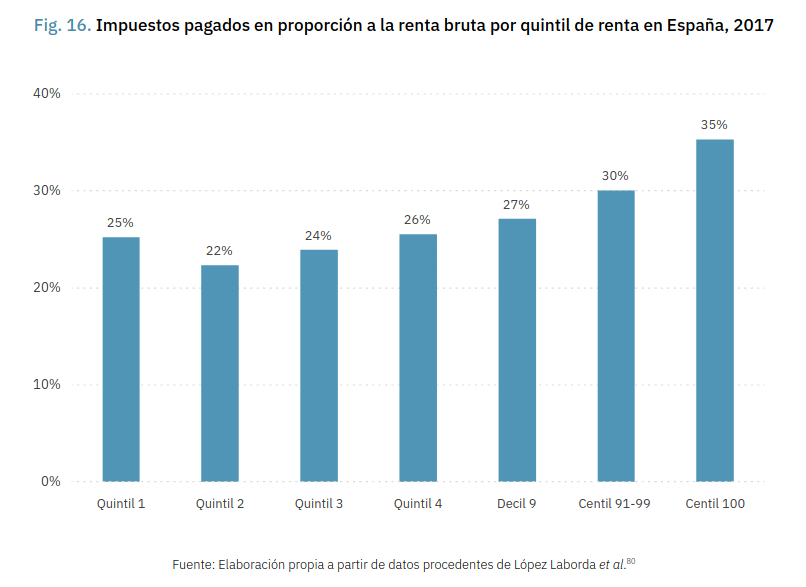
\includegraphics[width=4.89861in,height=2.72639in]{png/image1.png}

\emph{Fuente: Ministerio de Presidencia a partir de López Laborda et
al.}

La Grafica 1 muestra la falta de progresividad final del sistema

\textbf{El papel de las prestaciones públicas}

Como hemos visto, el sistema tributario no es eficaz para luchar contra
la desigualdad. De hecho, son las prestaciones públicas (Transferencias)
las que, en España y en muchos países consiguen la reducción del índice
de Gini. En el caso de España un 93\% de la reducción de este índice es
debido a las prestaciones sociales frente al 7\% que se debe al sistema
fiscal (Laborda, Marín y Onrubia, 2017) tal y como recoge el también el
Documento de Estrategia España 2050. La práctica totalidad de ese 37\%
de reducción del índice Gini se consigue mediante las transferencias
como se aprecia si comparamos las Gráficas 2 y 3.

\emph{Gráfica 2. Reducción de la desigualdad en España como resultado
del sistema de prestaciones e impuestos}

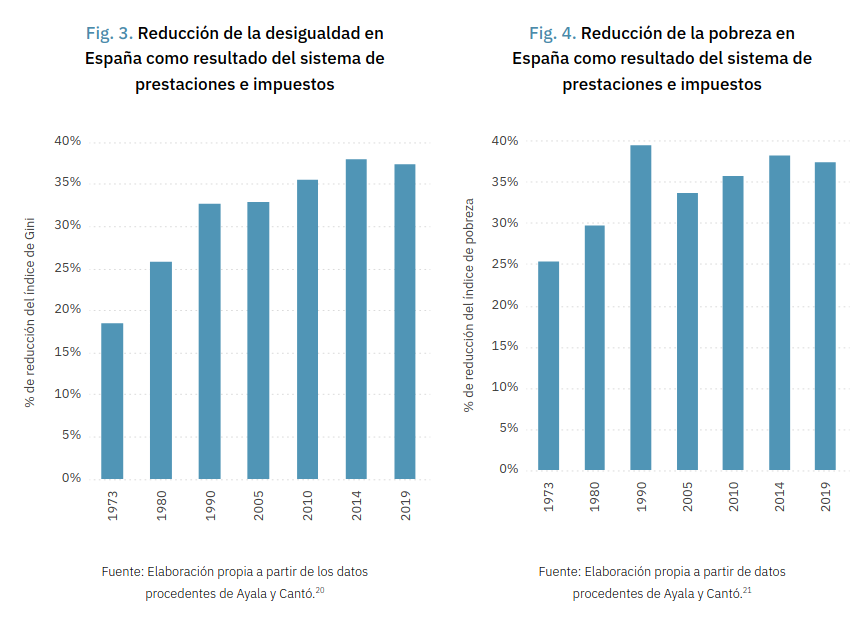
\includegraphics[width=5.1125in,height=3.15069in]{png/image2.png}
\emph{Fuente: Ministerio de Presidencia a partir de Ayala y Canto.}

\emph{Gráfica 3. Reducción de la pobreza en España como resultado de
prestaciones e impuestos}

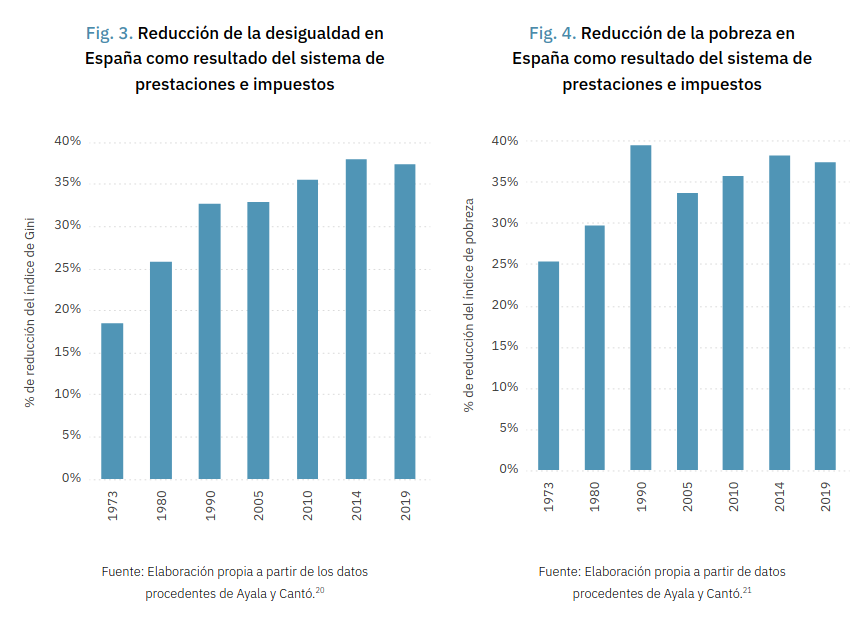
\includegraphics[width=4.65764in,height=3.39167in]{png/image2.png}
\emph{Fuente: Ministerio de Presidencia a partir de Ayala y Cantó}

\emph{Gráfica 4: Reducción de la desigualdad (Gini) por las
transferencias sociales (2019)}

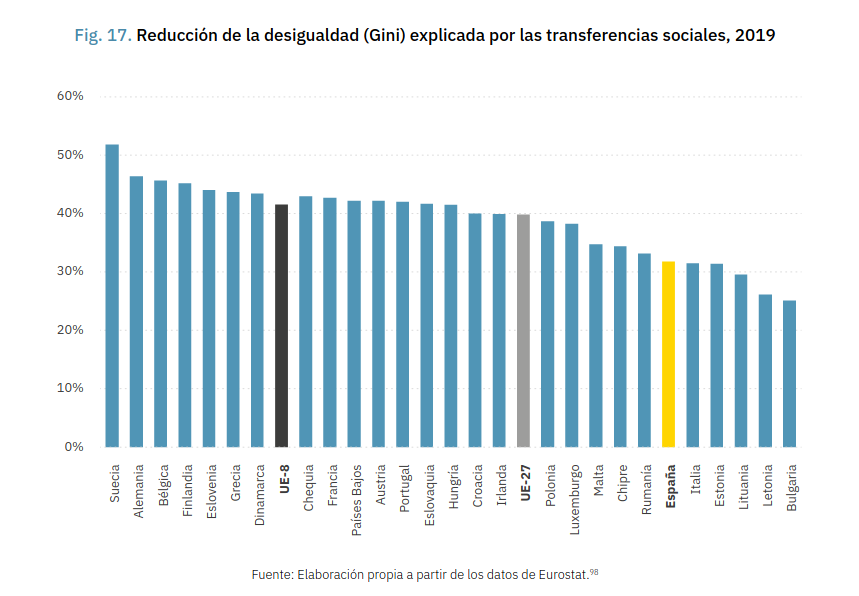
\includegraphics[width=5.92153in,height=3.62361in]{png/image3.png}
\emph{Fuente: Ministerio de Presidencia a partir Eurostat}

A la vista de los datos es lógico que las conclusiones que defienda un
think-tan liberal como el Institut Ostrom sobre el carácter regresivo
del sistema tributario español coincidas con las del documento de
estrategia del propio gobierno socialdemócrata. Otra cuestión son las
propuestas.

\hypertarget{el-ejemplo-del-tigre-celta}{%
\subsubsection*{El ejemplo del Tigre
Celta**}\label{el-ejemplo-del-tigre-celta}}
\addcontentsline{toc}{subsubsection}{El ejemplo del Tigre Celta**}

En el discurso liberal siempre aparece el paradigmático caso de Irlanda.
Este Estado europeo dispone de uno de los sistemas fiscales más
atractivos de la OCDE siendo la política de ``rebaja de impuestos'' para
grandes corporaciones su característica principal. Estamos un campeón de
la ``competencia fiscal''.

En comparación con España, la reducción de desigualdad en puntos de Gini
es muy superior pese a recaudar alrededor de 10 puntos menos sobre su
PIB (ver Gráfica 4). Los analistas, sobre todo los de inclinación
liberal, no dudan en achacar este éxito a un sistema tributario más
centrado en los impuestos directos que los indirectos. Se decantan por
la neutralidad sacrificando la progresividad lo que les proporciona una
mayor eficiencia. Así recaudan más y pueden reducir la pobreza mediante
transferencias.

No obstante, en estos últimos días (diciembre de 2022) se ha cerrado el
acuerdo en el seno de la UE para la aprobación de una Directiva que
recoge el plan de la OCDE de fijar un Impuesto de Sociedades mínimo del
15\%, Irlanda ha mantenido su tipo en un 12,5\%. La medida afectará en
2.000 millones a la recaudación, pero seguirá aplicando, entre otras
medidas, una deducción fiscal efectiva de hasta un 37,5\%. (Faes, 2022).

\textbf{La conclusión liberal: la neutralidad}

Pese a que los impuestos indirectos son más regresivos, su menor
distorsión en el mercado favorece el consumo viéndose beneficiada la
recaudación. Este incremento de recaudación nos permitiría reducir más
la desigualdad mediante las prestaciones sociales. Aunque haya
economistas liberales que defiendan esta que una mayor recaudación
permitiría mantener el Estado del bienestar a través del capítulo de
transferencias considerable, otros, más fieles la idea original del
liberalismo, ven la oportunidad para reducir la presión fiscal o hacer
frente a la deuda pública atendiendo a los principios de equilibrio
presupuestario y neutralidad.

\hypertarget{los-principios-en-los-nuevos-impuestos-excepcionales}{%
\section*{5 LOS PRINCIPIOS EN LOS NUEVOS IMPUESTOS
EXCEPCIONALES}\label{los-principios-en-los-nuevos-impuestos-excepcionales}}
\addcontentsline{toc}{section}{5 LOS PRINCIPIOS EN LOS NUEVOS IMPUESTOS
EXCEPCIONALES}

Las Cortes Generales han aprobado recientemente la Ley 38/2022, de 27 de
diciembre por la que se establecen tres nuevos impuestos, en principio,
provisionales. Uno para las grandes compañías energéticas, otro para la
banca y un tercero para las grandes fortunas.

En los tres casos se tratan de impuestos que tienen una vigencia
provisional de dos ejercicios (2023 y 2024) aunque la ley prevé una
posible renovación. La excepcionalidad de los tres impuestos no afecta
solo al periodo de aplicación, sino que, siguiendo el principio de
equilibrio, se acotan los posibles destinos de lo recaudado siendo éstos
coyunturales.

\hypertarget{gravamen-temporal-energuxe9tico}{%
\subsection{5.1 GRAVAMEN TEMPORAL
ENERGÉTICO}\label{gravamen-temporal-energuxe9tico}}

La nueva propuesta de impuestos supondrá un gravamen del 1,2\% sobre las
ventas para las grandes compañías energéticas con un importe neto
superior a los 1.000 millones de euros en 2019.

Se trata, por lo tanto, de un impuesto motivado sobre todo por el
principio de equidad, aunque se entienda como un impuesto proporcional a
partir de un mínimo y no puramente progresivo.

\textbf{La polémica (y la paradoja del principio de simplicidad)}

Las compañías han defendido que el impuesto se aplicase sobre los
beneficios mientras que el Gobierno ante la posibilidad de que éstos
sean camuflados (``cocinando'' las cifras) ha defendido en todo momento
que el impuesto se aplique sobre los ingresos. En este caso se da la
paradoja de que la Administración Tributaria, y no el administrado, es
la que teme a la complejidad de los cálculos y reclama para sí un modelo
simplicidad y transparencia.

\textbf{Destino determinado}

La Ley 38/2022 (artículo 1.11) se establece los fines a los que se
destinará la recaudación. Básicamente podrían resumirse en medidas
sociales especialmente la reducción de los efectos de la crisis
energéticas y medidas para mejorar la eficiencia o ahorro energético.

\hypertarget{gravamen-temporal-de-entidades-de-cruxe9dito-y-establecimientos-financieros-de-cruxe9dito}{%
\subsection*{5.2 GRAVAMEN TEMPORAL DE ENTIDADES DE CRÉDITO Y
ESTABLECIMIENTOS FINANCIEROS DE
CRÉDITO}\label{gravamen-temporal-de-entidades-de-cruxe9dito-y-establecimientos-financieros-de-cruxe9dito}}
\addcontentsline{toc}{subsection}{5.2 GRAVAMEN TEMPORAL DE ENTIDADES DE
CRÉDITO Y ESTABLECIMIENTOS FINANCIEROS DE CRÉDITO}

Se aplicará para aquellas entidades que en 2019 hayan superado en
ingresos por intereses y comisiones más de 800 millones de euros. El
gravamen temporal será del 4,8\% sobre las comisiones e intereses netos
de la banca.

Al igual que el anterior, se trata, por lo tanto, de un impuesto
motivado sobre todo por el principio de equidad siendo también
proporcional. Se aplica un gravamen fijo (impuesto directo proporcional)
a partir de un mínimo de ingresos.

Una de las polémicas en este impuesto se debe a la prohibición de
repercutir este impuesto a los clientes. La ley contempla sanciones y
designa a la CNMC para supervisar que no se produzca un encarecimiento
del crédito para compensar el pago del impuesto. Por su parte, el BCE se
ha posicionado a favor de considerar todos los costes (incluyendo los
fiscales) a la hora determinar los precios. De la repercusión o no en
los precios del impuesto dependería el carácter social pretendido. Para
el BCE está en cuestión el criterio o principio de eficiencia, para el
Gobierno, el de equidad.

\textbf{Destino determinado}

En la Ley 38/2022 (artículo 2.10) se especifica que el importe recaudado
será destinado a medidas para paliar el incremento de precios como
consecuencias de la guerra en Ucrania. Esta era una de las demandas del
Banco Central Europeo, que se destinasen a un fin concreto y excepcional
consecuencia de la situación , de nuevo el principio de suficiencia o
equilibrio presupuestario.

\hypertarget{impuesto-temporal-de-solidaridad-de-las-grandes-fortunas}{%
\subsection{5.3 IMPUESTO TEMPORAL DE SOLIDARIDAD DE LAS GRANDES
FORTUNAS}\label{impuesto-temporal-de-solidaridad-de-las-grandes-fortunas}}

A través de una enmienda parlamentaria se introdujo en la primera
propuesta de la que sería la ley 38/2022 un tercer impuesto directo y
personal sobre las grandes fortunas. Se aplicará en fortunas superiores
a 3 Millones de euros. Su cálculo será similar al del impuesto de
patrimonio (bienes y derechos, menos deudas y cargas), las mismas
exenciones y un mínimo exento de 700.000 euros. Los tipos a aplicar
serán los reflejado en la tabla siguiente:

\emph{Tabla1: Tarifa del impuesto temporal de solidaridad de las grandes
fortunas.}

\begin{longtable}[]{@{}
  >{\raggedright\arraybackslash}p{(\columnwidth - 6\tabcolsep) * \real{0.2329}}
  >{\raggedright\arraybackslash}p{(\columnwidth - 6\tabcolsep) * \real{0.2466}}
  >{\raggedright\arraybackslash}p{(\columnwidth - 6\tabcolsep) * \real{0.2466}}
  >{\raggedright\arraybackslash}p{(\columnwidth - 6\tabcolsep) * \real{0.2466}}@{}}
\toprule\noalign{}
\endhead
\bottomrule\noalign{}
\endlastfoot
BASE LIQUIDABLE

HASTA € & CUOTA

€ & RESTO BASE LIQ.

HASTA € & TIPO APLICABLE

\% \\
0 & 0 & 3 MILLONES & 0 \\
3M & 0 & 2.347.998,03 & 1,7 \\
5.347.998,03 & 39.915,97 & 5.347.998,03 & 2,1 \\
10.695.996,06 & 152.223,93 & En adelante\ldots{} & 3,5 \\
\end{longtable}

Vemos claramente que se trata de un impuesto directo progresivo basado
en una tarifa o escala de gravamen.

\textbf{Destino determinado}

De nuevo en la Ley (artículo 3.25) se determina como único destino de la
recaudación a ``políticas de apoyo a los más vulnerables''.

\textbf{Polémica}

En el borrador inicial no se contemplaba la aplicación del impuesto
sobre las participaciones accionariales en no residentes con activos en
España para evitar que el no residente eluda el gravamen. No se estaba
respetando el principio de equidad entendido como la generalización de
la carga tributaria algo que se entendía como de dudosa
constitucionalidad.

\hypertarget{sobre-la-suficiencia}{%
\subsection*{5.4 SOBRE LA SUFICIENCIA}\label{sobre-la-suficiencia}}
\addcontentsline{toc}{subsection}{5.4 SOBRE LA SUFICIENCIA}

Tal como recoge el preámbulo de la ley, el dictamen del Banco Central
Europeo de 2 de noviembre de 2022 sobre la imposición de gravámenes
temporales «es necesaria una clara separación entre la cuenta
extraordinaria creada a partir de los ingresos procedentes de los
gravámenes y los recursos presupuestarios generales de las
administraciones públicas para evitar su utilización con fines de
saneamiento presupuestario general». El BCE se aferra a la idea de la
regla del equilibrio presupuestario o el principio de suficiencia pero
es evidente que estamos ante las circunstancias excepcionales que según
Peacock y Wiseman exigen una flexibilidad del sistema tributario.

\hypertarget{el-impuesto-sobre-el-patrimonio-y-las-bonificaciones-de-la-junta-de-andalucuxeda}{%
\subsection{5.5 El Impuesto sobre el Patrimonio y las bonificaciones de
la Junta de
Andalucía}\label{el-impuesto-sobre-el-patrimonio-y-las-bonificaciones-de-la-junta-de-andalucuxeda}}

Estas medidas del Gobierno de España van en el sentido contrario a las
tomadas por la Junta de Andalucía en materia impositiva en la recta
final de 2022. El Gobierno andaluz, por medio de Decreto-Ley (también
las autonomías usan y abusan de esta figura), han aprobado la
bonificación el 100\% del Impuesto del Patrimonio. En la argumentación,
curiosamente de igual manera, se apela a la actual situación actual de
inflación.

El Impuesto sobre le Patrimonio solo tiene su réplica en nuestro entorno
en países como algunos cantones de Suiza o en Noruega aunque con tipos
más bajos. De hecho se suprimió en Austria, Dinamarca y Alemania a
finales del siglo pasado y en Luxemburgo, Finlandia, Suecia y Francia
posteriormente.

Los analistas liberales, contrarios al Impuesto sobre le Patrimonio, ven
en este impuesto ``un encarecimiento del coste del capital de las
empresas, lo que penaliza el ahorro, la inversión, la productividad y el
crecimiento'' (Jiménez-Mausbach, 2022). Y un aliciente para el cambio de
domicilio fiscal y las políticas tendentes a la competencia fiscal

Los defensores de esta figura apelarán a la necesidad, de hecho en
España llegó a suprimirlo en 2008 y recuperarlo para hacer frente a la
crisis en 2011. Respecto a la deslocalización del ahorro a otras
regiones o Estados, culpabilizan a los gobiernos autonómicos que
aprueban bonificaciones o gobiernos nacionales que aprueban supresiones.

\hypertarget{conclusiones}{%
\section*{6 CONCLUSIONES}\label{conclusiones}}
\addcontentsline{toc}{section}{6 CONCLUSIONES}

Respecto a la compatibilidad de los principios, partimos de dos visiones
distintas que comparten, en el mejor de los casos, el objetivo de
reducir la desigualdad social o al menos, mejorar el nivel de vida de la
mayoría. Ambas intentarán asumir la mayoría de los principios clásicos
en la medida de lo posible, pero diferirán mayormente en la importancia
y la valoración de los principios de neutralidad y equidad (eficiencia y
progresividad). Para unos la neutralidad es fundamental puesto que
aporta eficiencia mientras que para otros no se puede sacrificar la
progresividad puesto que aporta justicia.

Por otra parte tenemos los tributos extrafiscales o pignouvianos que no
atienden a ninguno de estos principios el objetivo de corregir procesos
productivos o costumbres sociales que afectan, generalmente, al
medioambiente o también la salud en general.

Otro aspecto importante sobre el principio de equidad y la eficiencia en
si, es el carácter regresivo de nuestro sistema y su poca incidencia en
los objetivos de igualdad frente a las políticas de gasto.

En cuanto al marco legal sí que debemos anotar cierta evolución. Los
nuevos tributos quedan establecidos por leyes estatales o autonómicas
que nacen a partir de Directivas europeas previas. En nuestro sistema
fiscal conviven los proporcionales tributos locales heredados de las
antiguas contribuciones con las indicaciones de la política común
europea. Ejemplo de esta son los nuevos impuestos verdes, las
indicaciones del BCE y que acaban moldeando los nuevos impuestos
excepcionales con fines sociales o la imposición de un mínimo en el
impuesto de sociedades.

Una última conclusión de carácter más general sobre nuestro sistema
tributario. Debemos reconocer que si bien estamos lejos de acuerdos como
el impuesta mundial de Piketty, sí que existe un denominador común: la
evolución del sistema tributario sigue unos principios decididos por
instituciones supraestatales incluso cuando son iniciativa nacional.

\hypertarget{bibliografuxeda}{%
\section{7 BIBLIOGRAFÍA}\label{bibliografuxeda}}

\begin{itemize}
\item
  Boscá, J.E; Doménech, R y Ferri, J 2017. \emph{Estructura fiscal,
  crecimiento económico y bienestar.} BBVA
\item
  Faes, I. ``¿Porqué Irlanda mantendrá las empresa pese al tipo
  mínimo?''. \emph{Expansión} , 21/12/2022
\item
  Jiménez-Mausbach, M ``A vueltas con el\,Impuesto de Patrimonio y la
  armonización fiscal''. Economiadigital.es, 28/09/2022.
  \url{https://www.economiadigital.es/ideas/a-vueltas-con-el-impuesto-de-patrimonio-y-la-armonizacion-fiscal.html}
  Consulta: 03/01/2023, 13:25
\item
  Kox, H; Lejour, A 2005 ``Regulatory Heterogeneity as Obstacle for
  International Servicea Trade", CPB Discussion Paper, nª 49
\item
  Laborda, JL; Marín, C. y Onrubia, J 2016. ``Observatorio sobre el
  reparto de los impuestos y las prestaciones monetarias entre los
  hogares españoles. FEDEA
\item
  Martínez-Gil X. 2018 ``Beneficios fiscales, ¿beneficios para quién?''.
  Plataforma por una fiscalidad
  justa.\url{https://www.elsaltodiario.com/justicia-fiscal/beneficios-fiscales-perdidas-sociales}
  Consulta: 28/12/2022, 19:20
\item
  Oficina nacional de prospectiva y estrategia. Ministerio de la
  Presidencia, 2021 ``Reducir la pobreza y la desigualdad y reactivar el
  ascensor social (Objetivo)'' en ``Estrategia España
  2050''h\href{https://www.lamoncloa.gob.es/presidente/actividades/Documents/2021/200521-Estrategia_Espana_2050.pdf}{ttps://www.lamoncloa.gob.es/presidente/actividades/Documents/2021/200521-Estrategia\_Espana\_2050.pdf}
  Consultado el 2/01/2023, 13:25
\item
  Piketty, T. 2014 ``El capital en el siglo XXI'' Madrid: Fondo de
  cultura económica.
\item
  Rodríguez, A. \emph{et al.} 2018. \emph{Declaración de Granada.}
  \url{https://www.aedaf.es/Plataforma/DOC20180521_Documento\%20Granada\%20(18\%20mayo\%202018).pdf}
  Consulta: 29/12/2022, 18:25
\item
  Rossell Barellas, Anna, 2020, ``Hem d'apujar el impostos als rics?''
  en Jiménez-Mausbach, Martí, \emph{La resposta Liberal}, Barcelona:
  Editorial Base.
\end{itemize}

\hypertarget{legislaciuxf3n}{%
\section*{8 LEGISLACIÓN}\label{legislaciuxf3n}}
\addcontentsline{toc}{section}{8 LEGISLACIÓN}

\begin{itemize}
\item
  Ley 7/2022, de 8 de abril, de residuos y suelos contaminados para una
  economía circular. (BOE núm. 85, de 09 de abril de 2022)
\item
  Decreto-ley 7/2022, de 20 de septiembre, por el que se modifica la Ley
  5/2021, de 20 de octubre, de Tributos Cedidos de la Comunidad Autónoma
  de Andalucía, para paliar los efectos de la inflación mediante la
  deflactación del gravamen del Impuesto sobre la Renta de las Personas
  Físicas y para bonificar el Impuesto sobre el Patrimonio, se aprueba
  la supresión del gravamen para 2023 del canon de mejora de
  infraestructuras hidráulicas de interés de la Comunidad Autónoma de
  Andalucía, y se modifica el Texto Refundido de la Ley General de la
  Hacienda Pública de la Junta de Andalucía en materia de aplazamiento y
  fraccionamiento de ingresos de derecho público de la Comunidad
  Autónoma. (BOJA núm 182, de 21 de septiembre de 2022).
\item
  Ley 38/2022, de 27 de diciembre, para el establecimiento de gravámenes
  temporales energético y de entidades de crédito y establecimientos
  financieros de crédito y por la que se crea el impuesto temporal de
  solidaridad de las grandes fortunas, y se modifican determinadas
  normas tributarias.(BOE núm. 311, de 28 de diciembre de 2022)
\end{itemize}

\end{document}
